\documentclass[russian, 12pt]{beamer}
\usepackage{multicol}
\usepackage[T2A,T1]{fontenc}
\usepackage[utf8]{inputenc}
\setcounter{secnumdepth}{3}
\setcounter{tocdepth}{3}
\usepackage{amsmath}
\usepackage{amssymb}
\usepackage{graphicx}
\usepackage{paratype}
\usepackage{hyperref}
\usepackage{xcolor}
\usepackage{listings}

\definecolor{codegreen}{rgb}{0,0.6,0}
\definecolor{codegray}{rgb}{0.5,0.5,0.5}
\definecolor{codepurple}{rgb}{0.58,0,0.82}
\definecolor{backcolour}{rgb}{0.95,0.95,0.92}

\lstdefinestyle{mystyle}{
    backgroundcolor=\color{backcolour},   
    commentstyle=\color{codegreen},
    keywordstyle=\color{magenta},
    numberstyle=\tiny\color{codegray},
    stringstyle=\color{codepurple},
    basicstyle=\ttfamily\footnotesize,
    breakatwhitespace=false,         
    breaklines=true,                 
    captionpos=b,                    
    keepspaces=true,                 
    numbers=left,                    
    numbersep=5pt,                  
    showspaces=false,                
    showstringspaces=false,
    showtabs=false,                  
    tabsize=2
}

\newcommand{\R}{\mathbb{R}}
\newcommand{\A}{\mathcal{A}}
\newcommand{\red}[1]{\textcolor{red!85!black}{{#1}}}
\renewcommand{\sp}[1]{\mathrm{sp}\left\{{{#1}}\right\}}
% Syntax: \colorboxed[<color model>]{<color specification>}{<math formula>}
\newcommand*{\colorboxed}{}
\def\colorboxed#1#{%
  \colorboxedAux{#1}%
} 
\newcommand*{\colorboxedAux}[3]{%
  % #1: optional argument for color model
  % #2: color specification
  % #3: formula
  \begingroup
    \colorlet{cb@saved}{.}%
    \color#1{#2}%
    \boxed{%
      \color{cb@saved}%
      #3%
    }%
  \endgroup
}

\makeatletter
\usepackage{tikz}
\usepackage{pgfplots}
% Remove warning about running in backwards compatibility mode
\pgfplotsset{compat=1.17}
\usepackage[all,cmtip]{xy}
\usetheme{Pittsburgh}
\usefonttheme{professionalfonts}
\setbeamercovered{transparent}
\setbeamertemplate{navigation symbols}{%
  \hspace{3.8em}%
  \vspace{0.5em}%
  \usebeamercolor[fg]{structure}%
  \usebeamerfont{subtitle}%
  \insertframenumber%
}
\makeatother

\usepackage{babel}

\title{Введение. Основные понятия.}
\subtitle{Алгоритмы и структуры данных}
\author{
  Мулюгин Н.\texorpdfstring{\thinspace}{Lg}В.
  \and
  Кузнецов М.\texorpdfstring{\thinspace}{Lg}А.
  }
\date{03.09.2022}

\begin{document}

\begin{frame}
\titlepage
\end{frame}
%%%%%%%%%%%%%%%%%%%%%%%%%%%%%%%%%%%%%%%%%%%%%%%%%%%%%%%%%%%%%%%%%%%%%%%%%%%%%%%
\begin{frame}
\frametitle{Информационные источники}
  \begin{itemize}
    \item [1] А. В. Столяров. Введение в профессию.\\
      http://stolyarov.info\\[0.5cm]

    \item [2] К. Владимиров.\\
    youtube.com/channel/UCvmBEbr9NZt7UEh9doI7$\_$A\\[0.5cm]

    \item [3] Ю. Окуловский.\\ 
    https://ulearn.me/

  \end{itemize}
\end{frame}
%%%%%%%%%%%%%%%%%%%%%%%%%%%%%%%%%%%%%%%%%%%%%%%%%%%%%%%%%%%%%%%%%%%%%%%%%%%%%%%
\begin{frame}
\frametitle{Информационные источники}
  \begin{itemize}
    \item [4] Томас Х. Кормен. Алгоритмы: построение и анализ.\\[0.5cm]

    \item [5] Томас Х. Кормен. Алгоритмы. Вводный курс.\\[0.5cm]

    \item [6] Род Стивенс. Алгоритмы. Теория и практическое применение.\\[0.5cm]
    
    \item [7] Никлаус Вирт. Алгоритмы и структуры данных.\\[0.5cm]
    
    \item [8] Д. Кнут. Искусство программирования.

  \end{itemize}
\end{frame}
%%%%%%%%%%%%%%%%%%%%%%%%%%%%%%%%%%%%%%%%%%%%%%%%%%%%%%%%%%%%%%%%%%%%%%%%%%%%%%%
\begin{frame}
\frametitle{Алгоритм}
\textbf{Алгоритм} представляет собой набор правил преобразования исходных данных(input) 
в выходные(output).\\[0.2cm]
Алгоритмы строятся для решения \textbf{вычислительных задач}.\\[0.2cm]
\textbf{Свойства} алгоритма:\\[0.2cm]
обязательные \hspace{3cm} необязательные
\begin{multicols}{2}
\begin{itemize}
  \item [1] Конечность.\\[0.3cm]

  \item [2] Дискретность.\\[0.3cm]

  \item [3] Определенность.\\[0.3cm]
  
  \item [4] Правильность. \\[0.3cm]
  
  \item [5] Завершаемость. \\[0.3cm]
  
  \item [5] Массовость. \\

\end{itemize}
\end{multicols}
\end{frame}
%%%%%%%%%%%%%%%%%%%%%%%%%%%%%%%%%%%%%%%%%%%%%%%%%%%%%%%%%%%%%%%%%%%%%%%%%%%%%%%
\begin{frame}
\frametitle{Сложность алгоритма}
\textbf{Время работы} алгоритма - 
число элементарных операций, которые он выполняет.\\[0.3cm]
\textbf{Время работы алгоритма в худшем случае (временная сложность)} - 
максимальное время работы для входов данного размера. \\[0.3cm]
\textbf{Асимптотическая сложность алгоритма} - 
оценка, характеризующая вид зависимости времени работы алгоритма от длины входа.

\end{frame}
%%%%%%%%%%%%%%%%%%%%%%%%%%%%%%%%%%%%%%%%%%%%%%%%%%%%%%%%%%%%%%%%%%%%%%%%%%%%%%%
\lstset{style=mystyle}
\begin{frame}
\frametitle{Сложность алгоритма}
\lstinputlisting[language=C++]{code/complex_1.cpp}
\end{frame}
%%%%%%%%%%%%%%%%%%%%%%%%%%%%%%%%%%%%%%%%%%%%%%%%%%%%%%%%%%%%%%%%%%%%%%%%%%%%%%%
\begin{frame}
\frametitle{Оценка сложности алгоритма}
\begin{figure}
  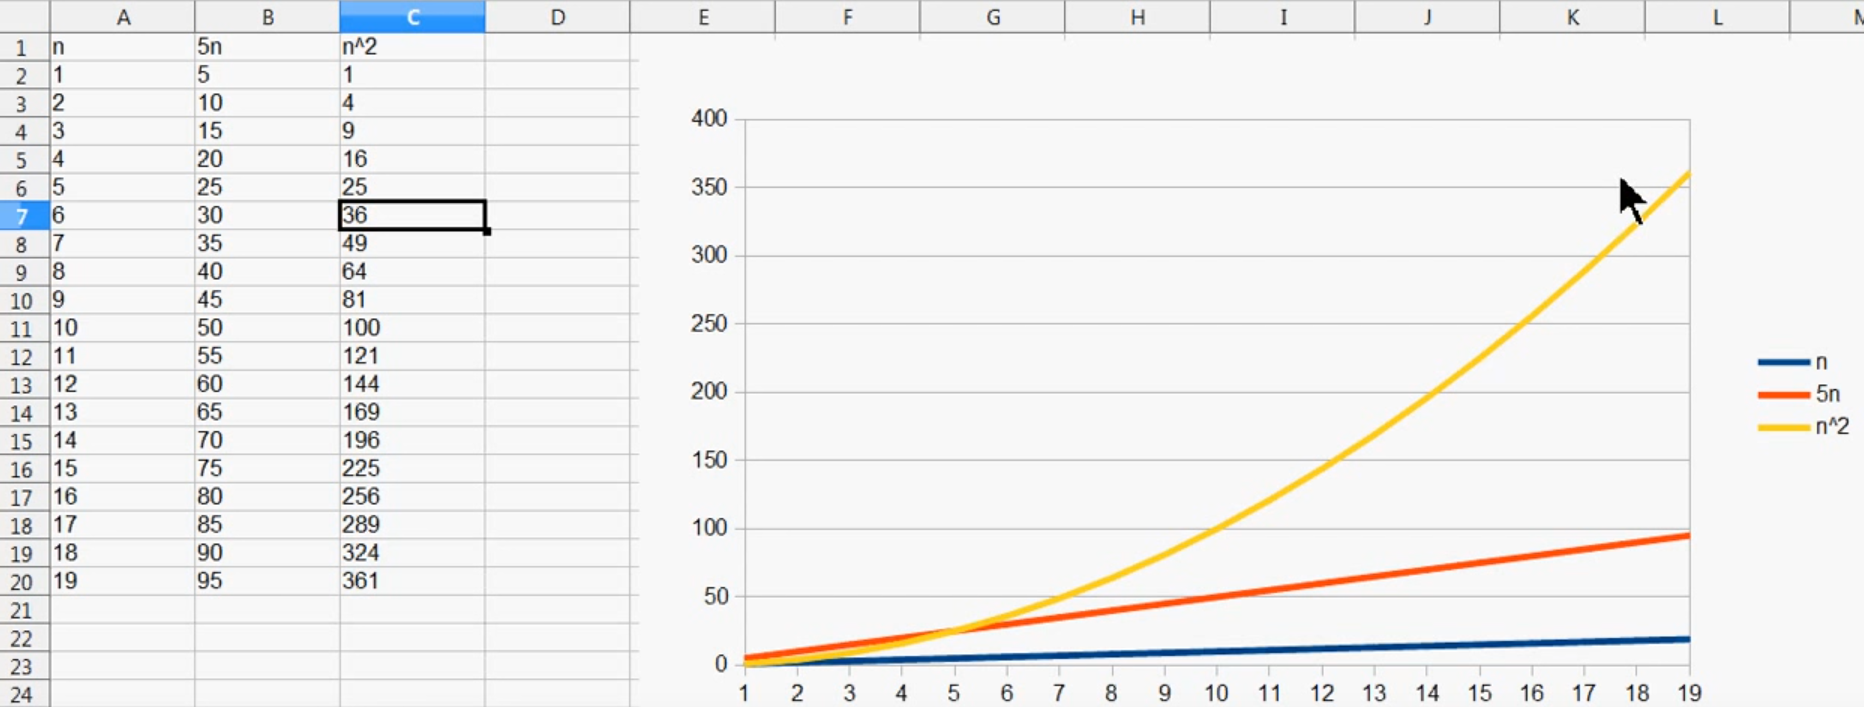
\includegraphics[width=\linewidth, height=5cm]{img/scal_1.png}
  %\caption{A boat.}
  %\label{fig:boat1}
\end{figure}
\end{frame}
%%%%%%%%%%%%%%%%%%%%%%%%%%%%%%%%%%%%%%%%%%%%%%%%%%%%%%%%%%%%%%%%%%%%%%%%%%%%%%%
\begin{frame}
\frametitle{Оценка сложности алгоритма}
\begin{figure}
  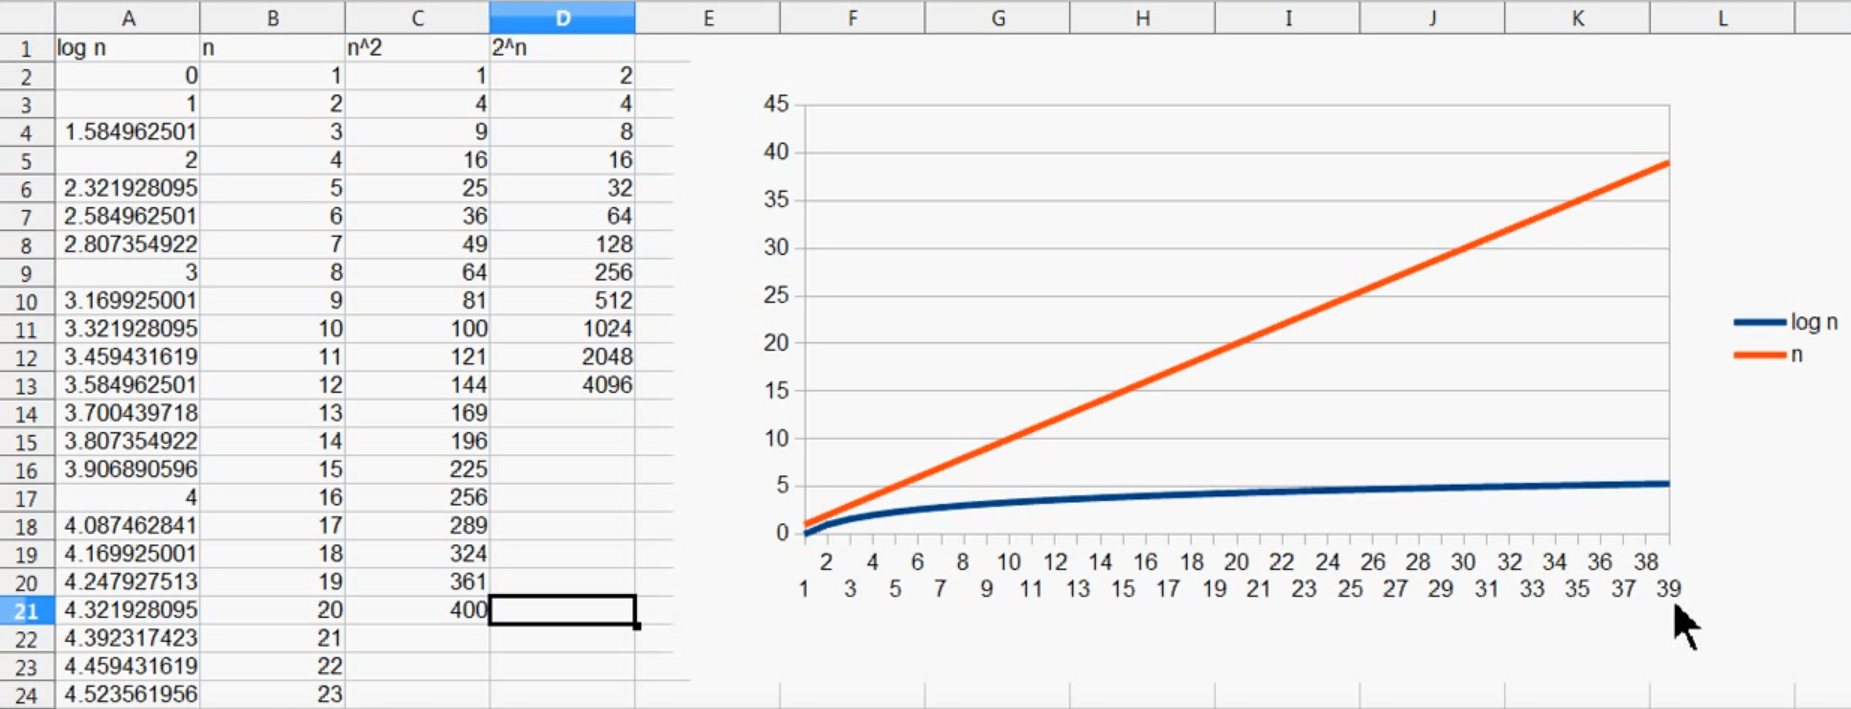
\includegraphics[width=\linewidth, height=5cm]{img/scal_2.png}
  %\caption{A boat.}
  %\label{fig:boat1}
\end{figure}
\end{frame}
%%%%%%%%%%%%%%%%%%%%%%%%%%%%%%%%%%%%%%%%%%%%%%%%%%%%%%%%%%%%%%%%%%%%%%%%%%%%%%%
\begin{frame}
\frametitle{Оценка сложности алгоритма}
\begin{figure}
  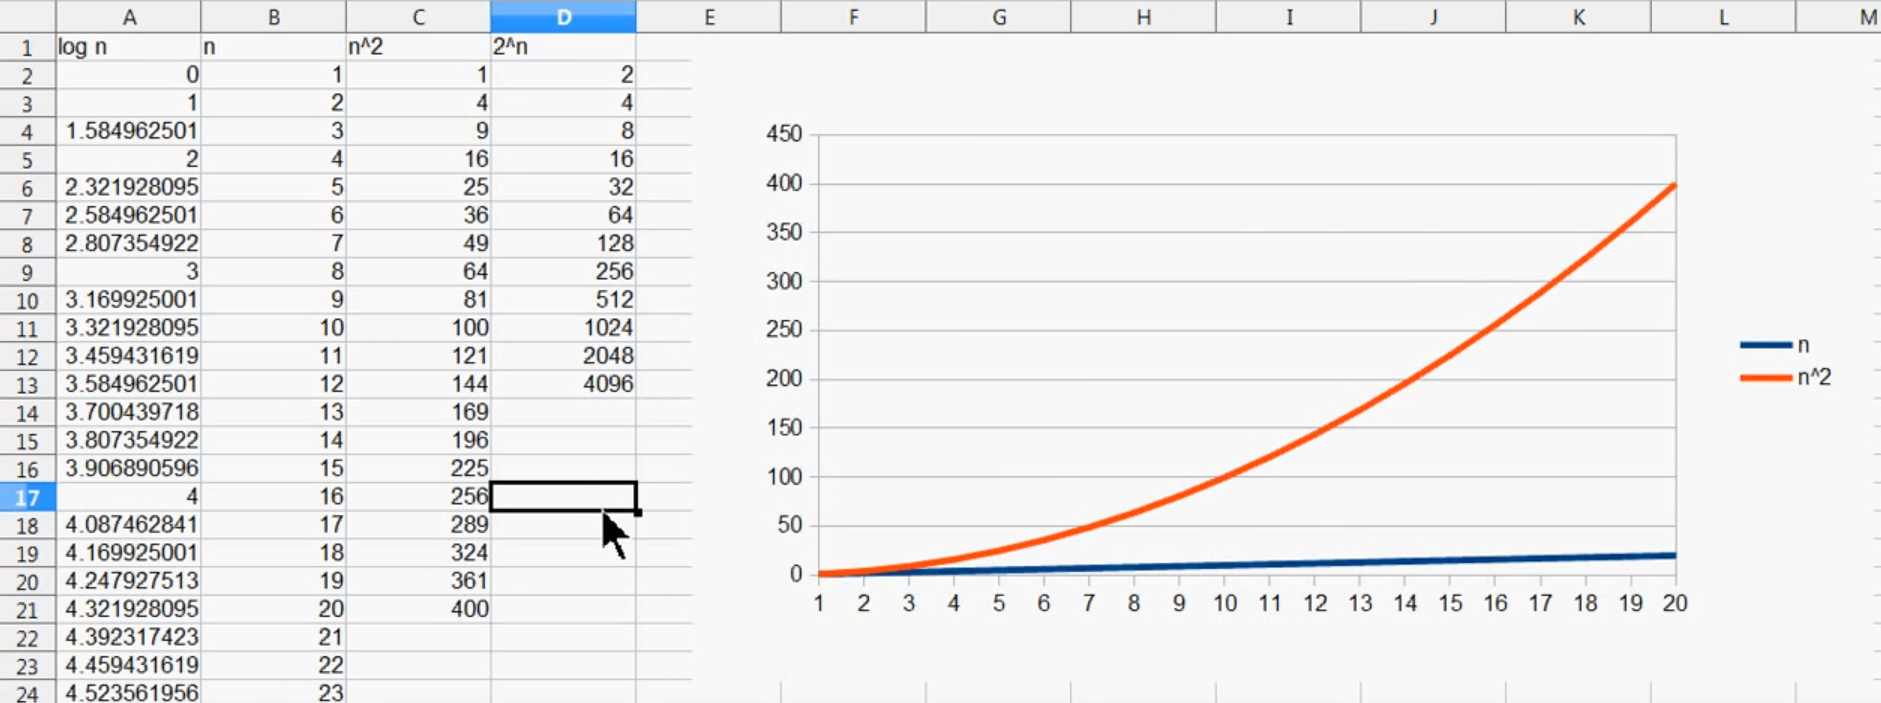
\includegraphics[width=\linewidth, height=5cm]{img/scal_3.png}
  %\caption{A boat.}
  %\label{fig:boat1}
\end{figure}
\end{frame}
%%%%%%%%%%%%%%%%%%%%%%%%%%%%%%%%%%%%%%%%%%%%%%%%%%%%%%%%%%%%%%%%%%%%%%%%%%%%%%%
\begin{frame}
\frametitle{Оценка сложности алгоритма}
\begin{figure}
  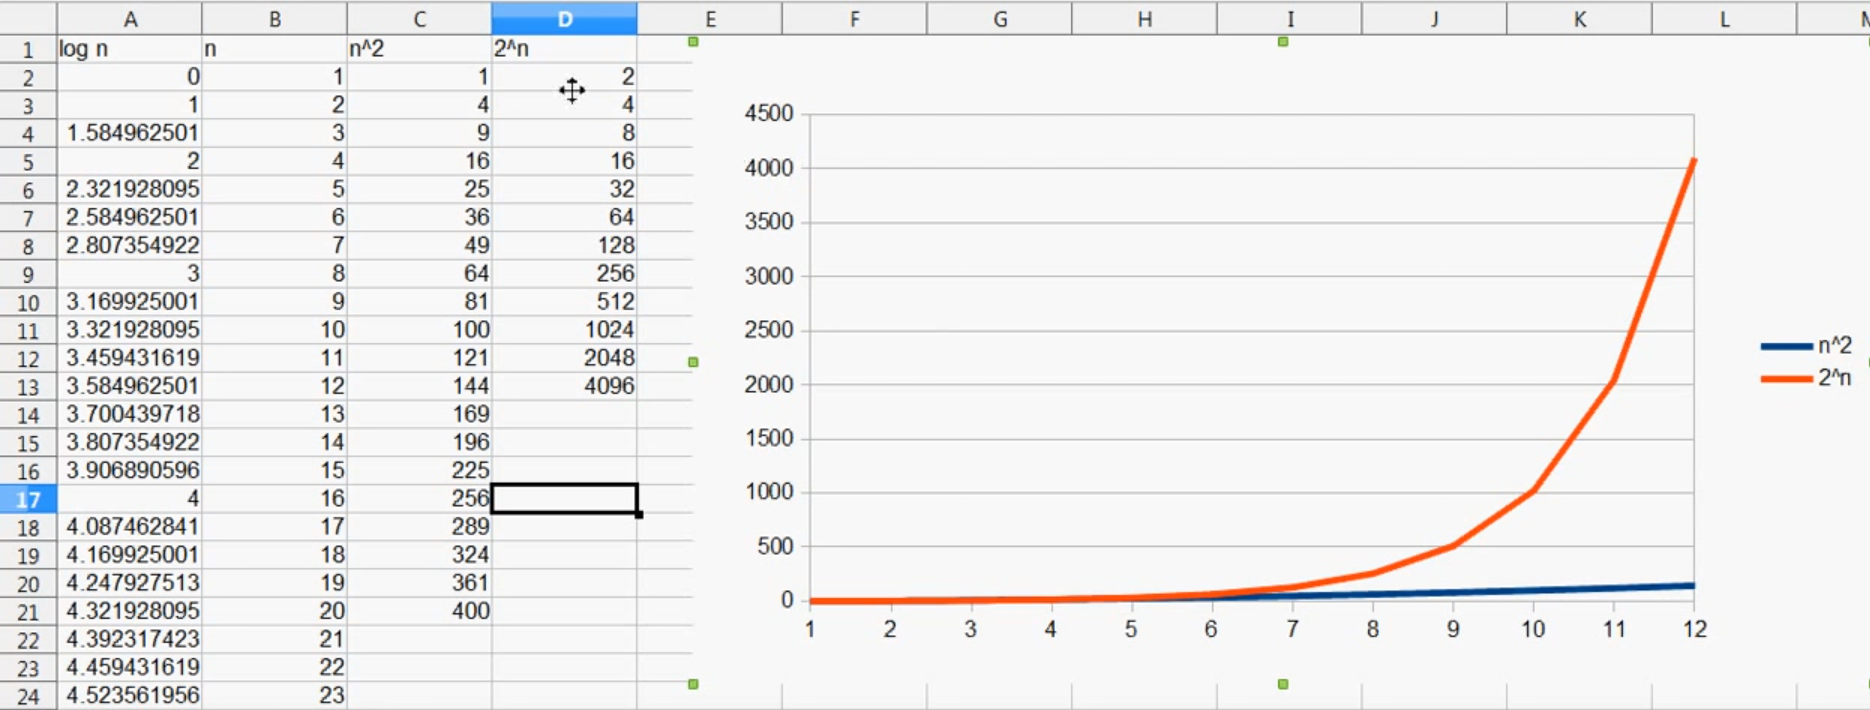
\includegraphics[width=\linewidth, height=5cm]{img/scal_4.png}
  %\caption{A boat.}
  %\label{fig:boat1}
\end{figure}
\end{frame}
%%%%%%%%%%%%%%%%%%%%%%%%%%%%%%%%%%%%%%%%%%%%%%%%%%%%%%%%%%%%%%%%%%%%%%%%%%%%%%%
\begin{frame}
\frametitle{O-символика}
%I
\begin{equation*}
\text{f(n) = o(g(n))}
  \begin{array}{l}
  \forall\text{k > 0}\;\exists\text{n}_0\;  \forall \text{n >}\text{n}_0  \\
  \text{f(n) < k $\cdot$ g(n)}
  \end{array}
\Leftrightarrow
\lim_{n\rightarrow\infty}\frac{\text{f(n)}}{\text{g(n)}}=\text{0}
\hspace{0.49cm}
\text{f(n) $\prec$ g(n)}
\end{equation*}
\vspace{0.3cm}
%II
\begin{equation*}
\text{f(n) = O(g(n))}
  \begin{array}{l}
    \exists\text{k > 0}\;\exists\text{n}_0\;  \forall \text{n >}\text{n}_0  \\
    \text{f(n) < k $\cdot$ g(n)}
  \end{array}
\Leftrightarrow
\lim_{n\rightarrow\infty}\frac{\text{f(n)}}{\text{g(n)}}<\infty
\hspace{0.25cm}
\text{f(n) $\preceq$ g(n)}
\end{equation*}
\vspace{0.3cm}
%III
\begin{equation*}
\text{f(n) = $\Theta$(g(n))}
%\hspace{0.2cm}
  \begin{array}{l}
    \exists\text{k}_1\text{k}_2 >\text{0}\;\exists\text{n}_0\hspace{0.5cm}\\
    \forall \text{n >}\text{n}_0\\
    \text{k}_1 \cdot \text{g(n)} < \text{f(n)}\\
    \text{f(n)} < \text{k}_2 \cdot \text{g(n)}
  \end{array}
\hspace{0.2cm}
\Leftarrow
\lim_{n\rightarrow\infty}\frac{\text{f(n)}}{\text{g(n)}}=\text{c}
\hspace{0.4cm}
\text{f(n) $\approx$ g(n)}
\end{equation*}
\end{frame}
%%%%%%%%%%%%%%%%%%%%%%%%%%%%%%%%%%%%%%%%%%%%%%%%%%%%%%%%%%%%%%%%%%%%%%%%%%%%%%%
\begin{frame}
\frametitle{Классы сложности}
Алгоритм со сложностью f(n) называется:
\begin{itemize}
  \item Если f $=\Theta(\log^kn)$: 
  логарифмическим при k=1, полилогарифмическим при k>1.\\[0.3cm]

  \item Если f $=\Theta(n)$: 
  линейным.\\[0.3cm]

  \item Если f $=\Theta(n\log^kn)$: 
  linearithmic при k=1, квазилинейным при k>1.\\[0.3cm]
  
  \item Если f $=\Theta(n^k)$: 
  полиномиальным, при k=2 квадратическим. \\[0.3cm]
  
  \item Если f $=\Theta(2^{n^k})$: 
  экспоненциальным. \\

\end{itemize}
\end{frame}
%%%%%%%%%%%%%%%%%%%%%%%%%%%%%%%%%%%%%%%%%%%%%%%%%%%%%%%%%%%%%%%%%%%%%%%%%%%%%%%
\begin{frame}
\frametitle{Рекурсивные алгоритмы}
Алгоритм это.
\end{frame}
%%%%%%%%%%%%%%%%%%%%%%%%%%%%%%%%%%%%%%%%%%%%%%%%%%%%%%%%%%%%%%%%%%%%%%%%%%%%%%%
\begin{frame}
\frametitle{Понятие типа}
Алгоритм это.
\end{frame}
%%%%%%%%%%%%%%%%%%%%%%%%%%%%%%%%%%%%%%%%%%%%%%%%%%%%%%%%%%%%%%%%%%%%%%%%%%%%%%%
\begin{frame}
\frametitle{Основные типы данных}
Алгоритм это.
\end{frame}
%%%%%%%%%%%%%%%%%%%%%%%%%%%%%%%%%%%%%%%%%%%%%%%%%%%%%%%%%%%%%%%%%%%%%%%%%%%%%%%
\begin{frame}
\frametitle{Представление числовых данных в памяти ЭВМ}
Представление числовых данных в памяти ЭВМ.
\end{frame}
%%%%%%%%%%%%%%%%%%%%%%%%%%%%%%%%%%%%%%%%%%%%%%%%%%%%%%%%%%%%%%%%%%%%%%%%%%%%%%%
\begin{frame}
\frametitle{Указатели}
Представление числовых данных в памяти ЭВМ.
\end{frame}
%%%%%%%%%%%%%%%%%%%%%%%%%%%%%%%%%%%%%%%%%%%%%%%%%%%%%%%%%%%%%%%%%%%%%%%%%%%%%%%
\begin{frame}
\frametitle{Порядок следования байтов}
Представление числовых данных в памяти ЭВМ.
\end{frame}
%%%%%%%%%%%%%%%%%%%%%%%%%%%%%%%%%%%%%%%%%%%%%%%%%%%%%%%%%%%%%%%%%%%%%%%%%%%%%%%
\begin{frame}
\frametitle{Структуры и объединения }
Представление числовых данных в памяти ЭВМ.
\end{frame}
%%%%%%%%%%%%%%%%%%%%%%%%%%%%%%%%%%%%%%%%%%%%%%%%%%%%%%%%%%%%%%%%%%%%%%%%%%%%%%%



\end{document}
